\documentclass[tikz,border=3pt,10pt]{standalone}

\usepackage{fontspec}
\usepackage{unicode-math}
\usepackage{pgfplots}
\pgfplotsset{compat=1.18}

\setmainfont{STIXTwoText-Regular.otf}[
  Path=../../../../../../../assets/fonts/,
  BoldFont=STIXTwoText-Bold.otf,
  ItalicFont=STIXTwoText-Italic.otf,
  BoldItalicFont=STIXTwoText-BoldItalic.otf
]
\setmathfont{STIXTwoMath.otf}[Path=../../../../../../../assets/fonts/]

\usetikzlibrary{backgrounds}

\definecolor{zoPlotBackground}{HTML}{FFF9E9}
\definecolor{zoPlotBorder}{HTML}{DFD7CA}
\definecolor{zoAxis}{HTML}{554F48}
\definecolor{zoText}{HTML}{3E3A35}
\definecolor{zoGraphMain}{HTML}{EF5350}
\definecolor{zoGraphStrong}{HTML}{BF4240}
\definecolor{zoReference}{HTML}{997918}

\pgfplotsset{
  zo axis/.style={
    width=12cm,
    height=7.5cm,
    scale only axis,
    axis equal image=false,
    enlargelimits=false,
    clip=true,
    clip mode=individual,
    axis lines=middle,
    grid=none,
    axis line style={draw=zoAxis,line width=0.8pt,<->},
    tick align=center,
    tickwidth=0.4mm,
    tick style={draw=zoAxis,line width=0.32pt},
    every axis plot/.append style={line cap=round,line join=round}
  },
  zo graph main/.style={
    draw=zoGraphMain,
    line width=1.2pt,
    solid,
    no marks
  },
  zo reference/.style={
    draw=zoReference,
    line width=0.8pt,
    densely dashed,
    no marks
  },
  zo point closed/.style={
    only marks,
    mark=*,
    mark size=2.2pt,
    draw=zoGraphMain,
    fill=zoGraphMain
  },
  zo point emphasized/.style={
    only marks,
    mark=*,
    mark size=2.8pt,
    draw=zoGraphStrong,
    fill=zoGraphStrong
  }
}

\tikzset{
  zo graph field/.style={
    show background rectangle,
    inner frame sep=4mm,
    background rectangle/.style={
      fill=zoPlotBackground,
      draw=zoPlotBorder,
      line width=0.45pt,
      rounded corners=2mm
    }
  },
  zo graph label/.style={
    text=zoText,
    font=\small
  },
  zo auxiliary label/.style={
    text=zoText,
    font=\small
  },
  zo point label/.style={
    text=zoText,
    font=\small
  }
}

\begin{document}
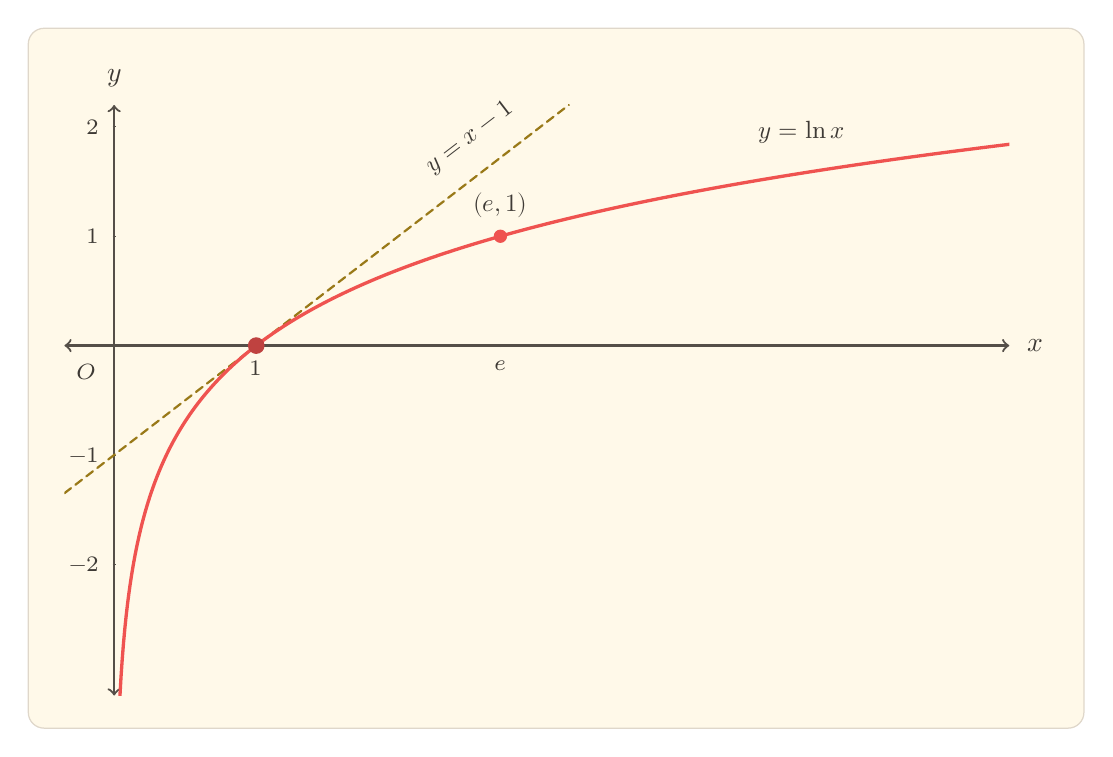
\begin{tikzpicture}[zo graph field]
  \begin{axis}[
    zo axis,
    xmin=-0.35,
    xmax=6.3,
    ymin=-3.2,
    ymax=2.2,
    xtick={1,2.718281828},
    ytick={-2,-1,1,2},
    xticklabel=\empty,
    yticklabel=\empty
  ]
    % Tiếp tuyến được vẽ trước đường cong chính và đi tới biên cửa sổ.
    \addplot[
      zo reference,
      domain=-0.35:3.2,
      samples=2
    ] {x-1};

    % Miền lấy mẫu chỉ nằm trong tập xác định x>0 và vượt nhẹ hai biên cắt.
    \addplot[
      zo graph main,
      domain=0.03:6.35,
      samples=700
    ] {ln(x)};

    \addplot[
      zo point emphasized
    ] coordinates {(1,0)};
    \addplot[
      zo point closed
    ] coordinates {(2.718281828,1)};

    \node[
      text=zoText,
      font=\footnotesize,
      anchor=north,
      yshift=-2pt
    ] at (axis cs:1,0) {$1$};
    \node[
      text=zoText,
      font=\footnotesize,
      anchor=north,
      yshift=-2pt
    ] at (axis cs:2.718281828,0) {$e$};
    \node[
      text=zoText,
      font=\footnotesize,
      anchor=east,
      xshift=-2pt
    ] at (axis cs:0,-2) {$-2$};
    \node[
      text=zoText,
      font=\footnotesize,
      anchor=east,
      xshift=-2pt
    ] at (axis cs:0,-1) {$-1$};
    \node[
      text=zoText,
      font=\footnotesize,
      anchor=east,
      xshift=-2pt
    ] at (axis cs:0,1) {$1$};
    \node[
      text=zoText,
      font=\footnotesize,
      anchor=east,
      xshift=-2pt
    ] at (axis cs:0,2) {$2$};

    \node[
      zo point label,
      anchor=south,
      xshift=0pt,
      yshift=3pt
    ] at (axis cs:2.718281828,1) {$(e,1)$};
    \node[
      zo graph label,
      anchor=south east,
      xshift=-2pt,
      yshift=4pt
    ] at (axis cs:5.25,{ln(5.25)}) {$y=\ln x$};

    % Nhãn tiếp tuyến nghiêng theo chính hướng hiển thị của đường.
    \path[
      draw=none
    ] (axis cs:2.1,1.1) -- (axis cs:3.05,2.05)
      node[
        zo auxiliary label,
        pos=0.58,
        sloped,
        above=5pt
      ] {$y=x-1$};

    \node[
      text=zoText,
      font=\normalsize,
      anchor=west,
      xshift=3pt
    ] at (axis cs:6.3,0) {$x$};
    \node[
      text=zoText,
      font=\normalsize,
      anchor=south,
      yshift=3pt
    ] at (axis cs:0,2.2) {$y$};
    \node[
      text=zoText,
      font=\footnotesize,
      anchor=north east,
      xshift=-3pt,
      yshift=-3pt
    ] at (axis cs:0,0) {$O$};
  \end{axis}
\end{tikzpicture}
\end{document}
